% !TEX TS-program = xepythontex



\documentclass[10pt,envcountsect,spanish]{beamer}


\newif\ifnotas
\notasfalse% Para no mostrar los globos
\notastrue % Para  mostrar los globos

\input ../preambulo.tex



%································ TITULO, AUTOR, ETC
\title{Tipos de Datos Abstractos Sin Orden}
\subtitle{Tecnología de la Programación}


\author[L. Daniel Hernández]{L. Daniel Hernández $<ldaniel@um.es>$}

\institute[ldaniel@um.es]{Dpto. Ingeniería de la Información  y las Comunicaciones\\ Universidad de Murcia\\ 19 de septiembre de 2023 \\\,\\\hrule} %	 \\ \today\\ \hrule}


\date[ldaniel@um.es]{ 
\vskip 1.25cm
%\vskip -1.25cm
%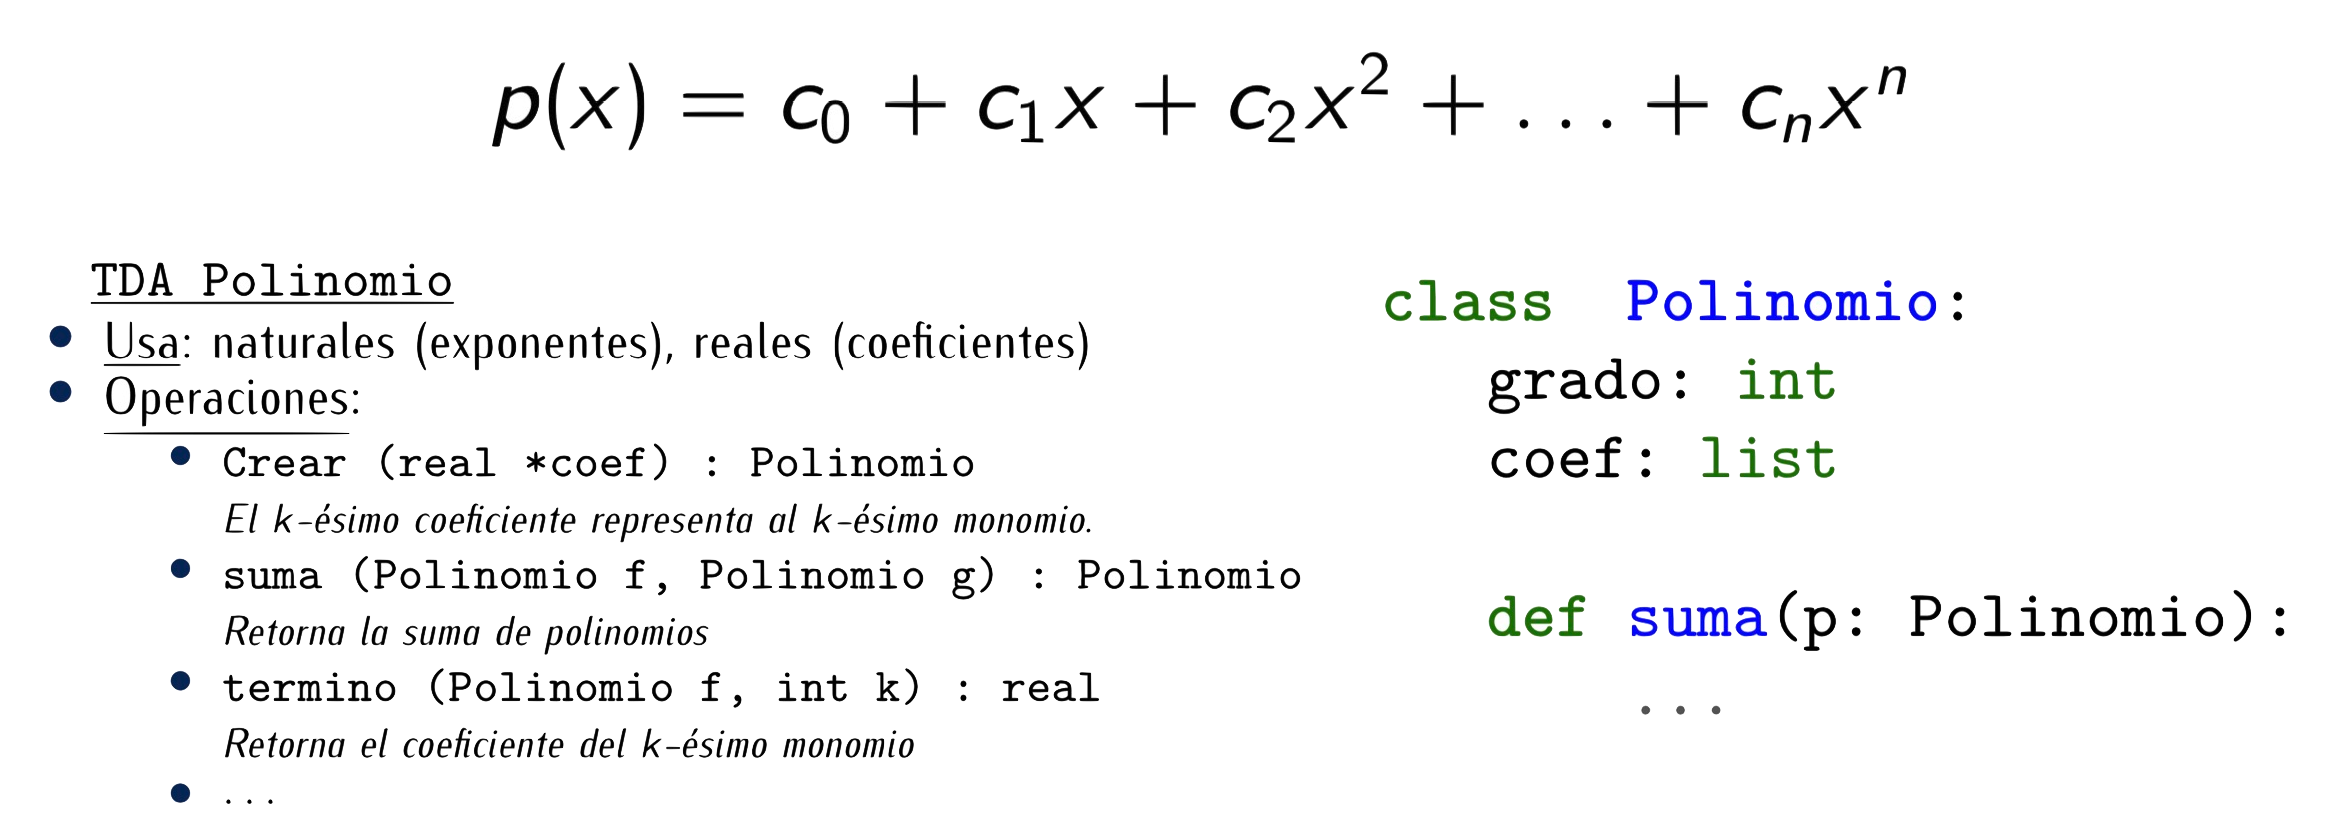
\includegraphics[width=.8\textwidth, height=.18\textheight]{fig/polinomio}
}

\graphicspath{{img/}}



%%%%%%%%%%%%%%%%%%%%%%%%%%%%%%%%%%
%%%%%%%%%%%%%%%%%%%%%%%%%%%%%%%%%%
%%%%%%%%%%%%%%%%%%%%%%%%%%%%%%%%%%
%%%%%%%%%%%%%%%%%%%%%%%%%%%%%%%%%%

%https://es.overleaf.com/learn/how-to/Writing_Markdown_in_LaTeX_Documents
\usepackage[hashEnumerators]{markdown}


%%%%%%%%%%%%%%%%%%%%%%%%%%%%%%%%%%
%%%%%%%%%%%%%%%%%%%%%%%%%%%%%%%%%%
%%%%%%%%%%%%%%%%%%%%%%%%%%%%%%%%%%
%%%%%%%%%%%%%%%%%%%%%%%%%%%%%%%%%%
\begin{document}

%\pgfdeclareimage[height=1cm]{logo}{logo.png}
%\logo{\pgfuseimage{logo}}



%--------------------------------------------------------------------------------
{\usebackgroundtemplate{%
  \includegraphics[width=\paperwidth,height=\paperheight]{../img/fondoUMUCompleto}}
\begin{frame}[b]
	\maketitle

\begin{tikzpicture}[overlay, remember picture]
\node[anchor=south west, %anchor is bottom left corner of the graphic
      xshift=.2\textwidth, %shifting around
      yshift=0.7cm] 
     at (current page.south west) %left bottom corner of the page
     {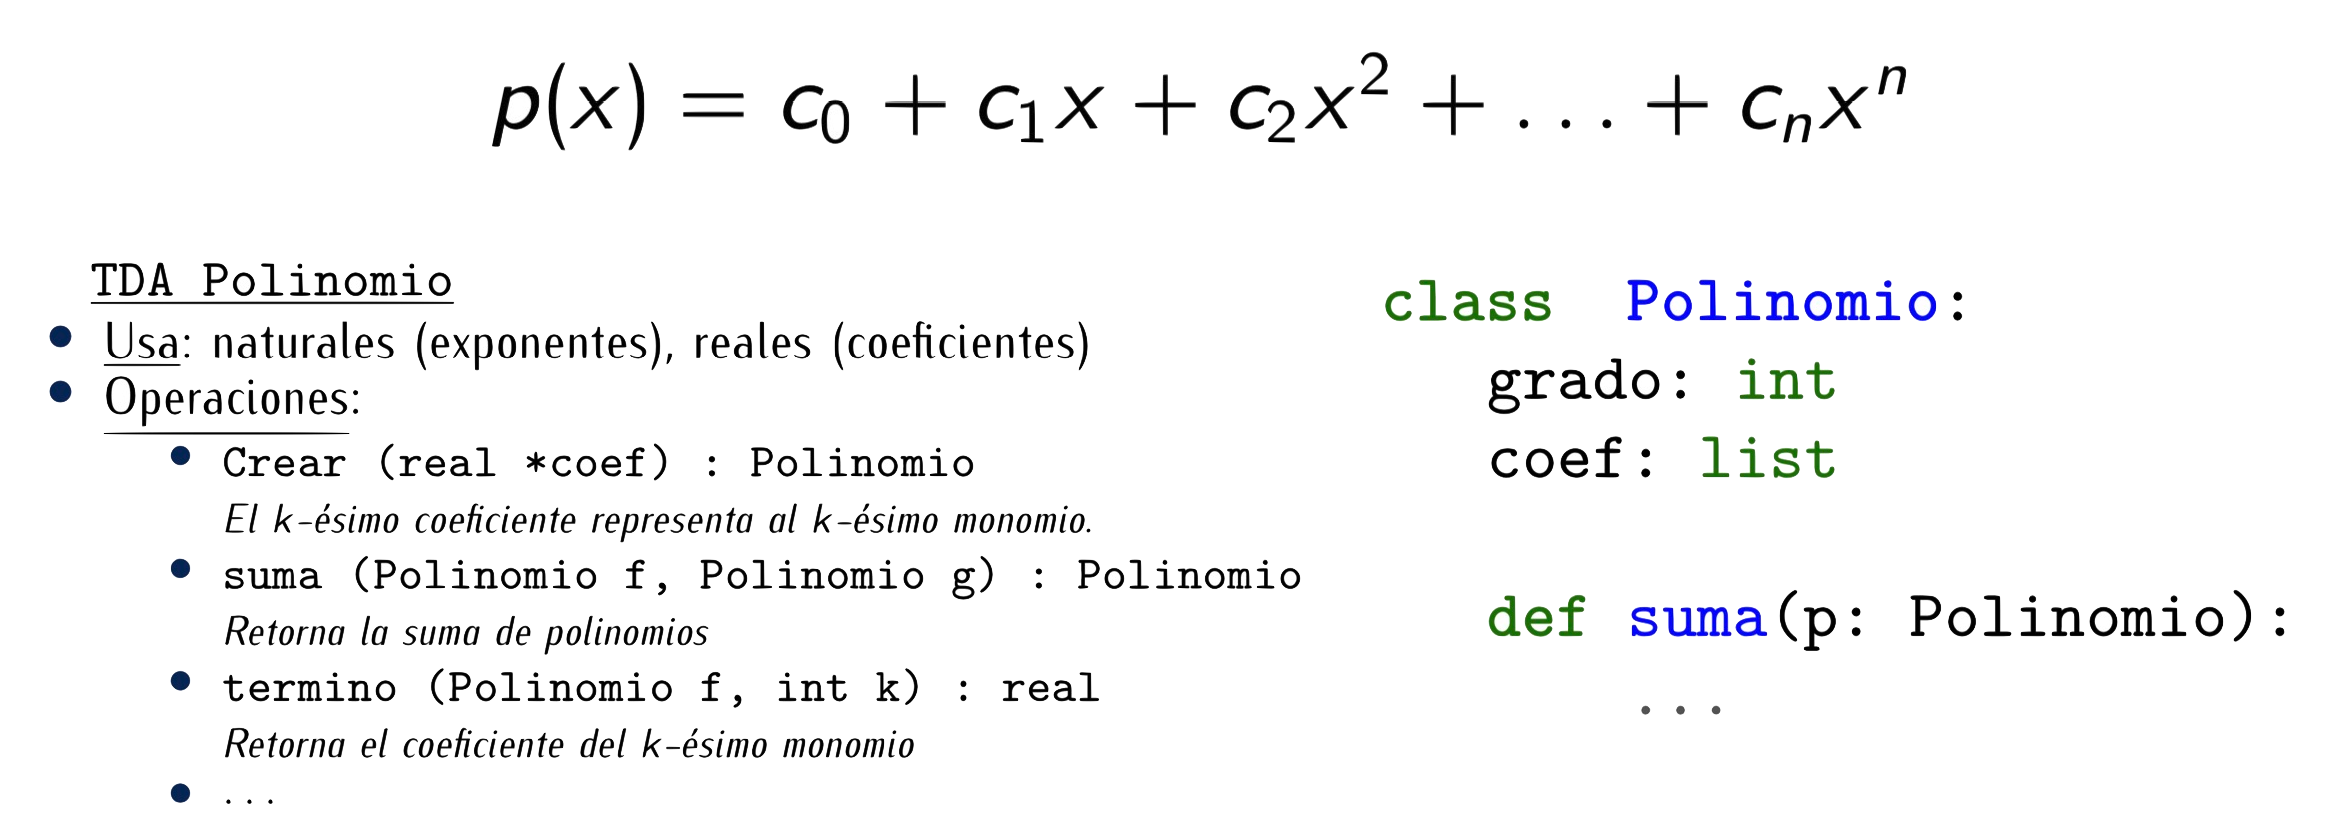
\includegraphics[width=.8\textwidth, height=.3\textheight]{fig/polinomio}}; 
\end{tikzpicture}
	
\end{frame}			% Transparencia: Título
}



%--------------------------------------------------------------------------------
%%%%%%%%%%%%%%%%%%%%%%%%%%%%%%%%%%
%%%%%%%%%%%%%%%%%%%%%%%%%%%%%%%%%%
\begin{frame}{Índice de Contenidos}\tableofcontents \end{frame}


%%%%%%%%%%%%%%%%%%%%%%%%%%%%%%%%%%%%%
%%%%%%%%%%%%%%%  SECTION   %%%%%%%%%%%%%%%
%%%%%%%%%%%%%%%%%%%%%%%%%%%%%%%%%%%%%
\section{TDAs sin orden}


%%%%%%%%%%%%%%%%%%%%%%%%%%%%%%%%%%
%%%%%%%%%%%%%%%%%%%%%%%%%%%%%%%%%%
\begin{frame}{Qué son los TDAs sin relación de orden}

\begin{itemize}%\setlength{\itemsep}{0mm}

\item Los TDAs sin relación de orden hacen referencia a contenedores donde no establecemos ningún criterio de ordenación entre los elementos que almacena. 

\item Ejemplos:
	\begin{itemize}
	\item La cesta de la compra en un supermercado.
	\item Las personas que están en un sala de espera, identificadas con un boleto.
	\end{itemize}

\item Podemos distinguir las bolsas (bag), conjuntos (set) y mapas (map).

\item Las operaciones generales que podemos definir en este tipo de contenedor, donde los objetos simplemente se almacenan son:
\begin{itemize}
\item Consultar el número de objetos que tiene el contenedor,
\item Determinar si el contenedor está vacío,
\item Añadir un nuevo objeto en el contenedor,
\item Informar si un objeto está en el contenedor (pertenencia),
\item Retirar un objeto del contenedor, y
\item Quitar todos los objetos de (limpiar) el contenedor.
\end{itemize}

\end{itemize}

\end{frame}



%%%%%%%%%%%%%%%%%%%%%%%%%%%%%%%%%%%%%
%%%%%%%%%%%%%%%  SECTION   %%%%%%%%%%%%%%%
%%%%%%%%%%%%%%%%%%%%%%%%%%%%%%%%%%%%%
\section{Bag}

%%%%%%%%%%%%%%%%%%%%%%%%%%%%%%%%%%
%%%%%%%%%%%%%%%%%%%%%%%%%%%%%%%%%%
\begin{frame}{Bag}

\begin{itemize}
\item Contenedor que almacena una colección de elementos (objetos o items) donde todos son del mismo tipo y no importa la posición dónde se almacenó cada uno ni el número de veces que aparecen.

\item Operaciones
\begin{itemize}
\item \cmn{Bag(): Bag}. Crea un nuevo \textit{bag}, inicialmente vacío.

\item \cmn{len(): int}. Retorna el número de elementos en el \textit{bag}.

Para una bag cualquiera $<a_0, a_1, \ldots, a_{n-1}>$ retornará el valor $n$.

\item \cmn{contains(item): bool}. Indica si el elemento \cmn{item} se encuentra en el \textit{bag}. Retorna \cm{True} si está contenido y \cm{False} si no está contenido.

\item \cmn{add(item): None}. Modifica el \textit{bag} añadiendo  el elemento \cmn{item} al \textit{bag}.

\item \cmn{remove(item): None}. Elimina y retorna la ocurrencia \cmn{item} del \textit{bag}. Lanza un error si el elemento no existe.

\item \cmn{iterator(): IteratorBag}. Crea y retorna un iterador para el \textit{bag}.
\end{itemize}

\end{itemize}

\end{frame}



%%%%%%%%%%%%%%%%%%%%%%%%%%%%%%%%%%%%%
%%%%%%%%%%%%%%%  SECTION   %%%%%%%%%%%%%%%
%%%%%%%%%%%%%%%%%%%%%%%%%%%%%%%%%%%%%
\section{Set}

%%%%%%%%%%%%%%%%%%%%%%%%%%%%%%%%%%
%%%%%%%%%%%%%%%%%%%%%%%%%%%%%%%%%%
\begin{frame}[allowframebreaks]{Set -}


\begin{itemize}%\setlength{\itemsep}{0mm} \footnotesize
\item Un Bag  donde \textbf{no se permite} la repetición de elementos. 

\item Operaciones:
\begin{itemize}
\item \cmn{Set(): Set}. Crea un nuevo conjunto, \textit{set}, inicialmente vacío.

\item \cmn{len(): int}. Retorna el número de elementos en el conjunto.

Para una lista cualquiera $<a_0, a_1, \ldots, a_{n-1}>$ retornará el valor $n$.

\item \cmn{contains(element): bool}. Indica si el elemento \cmn{element} se encuentra en el conjunto. Retorna \cm{True} si está contenido y \cm{False} si no está contenido.

\item \cmn{add(element): None}. Modifica el conjunto añadiendo  el elemento \cmn{element} al conjunto.

\item \cmn{remove(element): None}. Elimina el elemento \cmn{element} del conjunto. Lanza un error si el elemento no existe.


\item \cmn{iterator(): IteratorSet}: Crea y retorna un iterador para el conjunto.


\item \cmn{isSubsetOf(setB): bool}. Determina si un conjunto es subconjunto del conjunto dado. 

Un conjunto A es subconjunto de B si todos los elementos de A están en B.

\item \cmn{equal(setB): bool}. Determina si el conjunto es igual al conjunto dado. 

Dos conjuntos son iguales si ambos contienen el mismo número de elementos y todos los elementos del conjunto está en el conjunto B. Si ambos están vacíos entonces son iguales.


\item \cmn{union(setB): Set}. Retorna un nuevo conjunto que es la unión del conjunto con el conjunto dado.

La unión del conjunto A  con el conjunto de B es un nuevo conjunto que está formado por todos los elementos de A y todos los elementos de B que no están en A.


\item \cmn{difference(setB): Set}.  Retorna un nuevo conjunto que es la diferencia del conjunto con el conjunto dado.

La diferencia del conjunto A  con el conjunto de B es un nuevo conjunto que está formado por todos los elementos de A que no están en B.


\item \cmn{intersect(): Set}.  Retorna un nuevo conjunto que es la intersección del conjunto con el conjunto dado.

La intersección del conjunto A  con el conjunto de B es un nuevo conjunto que está formado por todos los elementos que están en A y también en B.

\end{itemize}

\item Notar que los 6 primeros operadores del TDA Set son análogos a los operadores del TDA Bag. Los restantes son operaciones bien conocidas de los conjuntos matemáticos.


\end{itemize}

\end{frame}




%%%%%%%%%%%%%%%%%%%%%%%%%%%%%%%%%%%%%
%%%%%%%%%%%%%%%  SECTION   %%%%%%%%%%%%%%%
%%%%%%%%%%%%%%%%%%%%%%%%%%%%%%%%%%%%%
\section{Map}

%%%%%%%%%%%%%%%%%%%%%%%%%%%%%%%%%%
%%%%%%%%%%%%%%%%%%%%%%%%%%%%%%%%%%
\begin{frame}{Map}


\begin{itemize}%\setlength{\itemsep}{0mm} \footnotesize
\item Colección de registros no repetidos donde cada uno consta de una clave y un valor. La clave debe ser comparable y es la que se utiliza para poder acceder al valor.

\item Ejemplos: tener las notas de los estudiantes por su identificador de estudiante, los datos fiscales por algún número de identificación, los datos de un conductor por el número de matricula de su vehículo,  etc ... 


\item Operaciones:

\begin{itemize}
\item \cmn{Map(): Map}. Crea un nuevo map vacío.

\item \cmn{len(): int}. Retorna el número de registros clave/valor que existen en el map..

\item \cmn{contains(key): bool}. Indica si la clave \cmn{key} se encuentra en el contenedor. Retorna \cm{True} si la clave está contenida y \cm{False} si no está contenida.


\item \cmn{remove(key): None}. Elimina el registro que tiene como clave el valor \cmn{key}. Lanza un error si el elemento no existe.


\item \cmn{add(key, value): None}. Modifica el map añadiendo el par \cmn{key/value} al contenedor. Si existiera un registro con la clave \cmn{key} se sustituye el par \cmn{key/value} existente por el nuevo par \cmn{key/value}. Retorna \cm{True} si la clave es nueva y \cm{False} si se realiza una sustitución.


\item \cmn{valueOf(key):  TipoValor}.  Retorna el valor asociado a la clave dada. La clave debe de existir en el Map.

\item \cmn{iterator(): IteratorMap}: Crea y retorna un iterador para el conjunto.
\end{itemize}
\end{itemize}

\end{frame}



%%%%%%%%%%%%%%%%%%%%%%%%%%%%%%%%%%%%%
%%%%%%%%%%%%%%%  SECTION   %%%%%%%%%%%%%%%
%%%%%%%%%%%%%%%%%%%%%%%%%%%%%%%%%%%%%
\section{Implementación}


%%%%%%%%%%%%%%%%%%%%%%%%%%%%%%%%%%
%%%%%%%%%%%%%%%%%%%%%%%%%%%%%%%%%%
\begin{frame}[fragile]{Cómo implementar los TDAs sin orden}

\begin{itemize}

\item \key{Estructuras integradas del lenguaje.}

\begin{itemize}
\item Algunas estructuras conocidas son: \cmn{array},  \cmn{list}, \cmn{tuple} y \cmn{dictionary}, \cmn{namedtuple}, \cmn{chainmap}, etc ...

\item Dependerá del lenguaje particular.


\item Python no tiene arrays.
\end{itemize}



\item \key{Estructuras enlazadas.} 

\begin{itemize}
\item Una estructura enlazada es aquella que se construye utilizando como estructura básica un \key{nodo}: 

\begin{pyverbatim}
struct Nodo
   valor: TDA
   referencia1 Nodo
   referencia2 Nodo
   ...
\end{pyverbatim}

\item Es una estructura construida por el programador.

\item Un nodo  sirve para representar muchos conceptos.

Ejemplo: elementos de un conjunto, los de una lista o los vértices de un árbol o un grafo.  

\item Distintos tipos de nodos nos sirve para implementar el mismo concepto de TDA. 

Ejemplo: un conjunto se puede implementar con un una referencia o con dos referencias.
\end{itemize}

\end{itemize}

\end{frame}


%%%%%%%%%%%%%%%%%%%%%%%%%%%%%%%%%%
%%%%%%%%%%%%%%%%%%%%%%%%%%%%%%%%%%
\section{Estructuras útiles de Python}
%%%%%%%%%%%%%%%%%%%%%%%%%%%%%%%%%%
%%%%%%%%%%%%%%%%%%%%%%%%%%%%%%%%%%


\begin{frame}{Estructuras útiles de Python}
%\small 
La estructuras de datos que presenta Python y que te pueden ayudar a implementar estos TDAs (y otros) son:

\setlist[itemize,1]{before*=\normalsize, leftmargin=\dimexpr 12pt}%,label=$\triangleleft$}
\begin{itemize}% \setlength{\itemsep}{0mm}
\item Rangos
\item Sets
\item Listas
\item Tuplas
\item Diccionarios
\end{itemize}

\


\


Consulte la documentación oficial sobre cada uno de estos tipos de datos.

\

Recuerda 
\begin{itemize}% \setlength{\itemsep}{0mm}
\item Un TDA no es una estructura de datos.
\item Un TDA no es una clase.
\end{itemize}


\end{frame}

\end{document}

%%%%%%%%%%%%%%%%%%%%%%%%%%%%%%%%%%
%%%%%%%%%%%%%%%%%%%%%%%%%%%%%%%%%%
\subsection{Abstracción de Datos}
%%%%%%%%%%%%%%%%%%%%%%%%%%%%%%%%%%
%%%%%%%%%%%%%%%%%%%%%%%%%%%%%%%%%%
\begin{frame}{Abstracción de Datos}
\begin{itemize}% \setlength{\itemsep}{0mm}
\item Existen 3 tipos (o niveles) de abstracción.
\item \key{Tipos de datos integrados}  (o fundamentales). Son los que ofrecen los lenguajes de programación.

\cm[magenta]{Ejemplo:} En \cm[red]{Python} se distinguen, entre otros\footnote[frame]{\url{https://docs.python.org/es/3/library/stdtypes.html}}:
\begin{itemize}
\item Los tipos de datos simples: numéricos (enteros, reales y complejos) y booleanos.
\item Los tipos de datos compuestos: cadena de caracteres (str), secuencias (rangos, listas y tuplas), mapas (diccionarios), conjuntos.
\end{itemize}


\item \key{Tipos de datos definidos por el usuario} o programador. Son los que pueden diseñar los programadores agrupando todos de datos fundamentales. 

\begin{itemize}
\item array, record, struct, \cm{class}
\end{itemize}

\item \key{Tipos de datos abstractos (TDA).} Construye modelos (matemáticos) usando agrupación de datos.

\begin{itemize}
\item No es lo mismo una estructura de datos formado por dos valores y operar con ellos que trabajar con vectores numéricos 2D con operaciones matemáticas (donde no importa la estructura).
\end{itemize}

\end{itemize}

\end{frame}




%%%%%%%%%%%%%%%%%%%%%%%%%%%%%%%%%%
%%%%%%%%%%%%%%%%%%%%%%%%%%%%%%%%%%
\section{Tipos de Datos Abstractos}
%%%%%%%%%%%%%%%%%%%%%%%%%%%%%%%%%%
%%%%%%%%%%%%%%%%%%%%%%%%%%%%%%%%%%
\begin{frame}{Tipos de Datos Abstractos}

\begin{itemize}
\item  Los \key{Tipos de Datos Abstractos} (TDA) son \textbf{modelos matemáticos} que constan de

\begin{itemize}
\item un nombre publico para 
\item identificar a un conjunto de datos (valores), junto con
\item un conjunto de operaciones bien definidas sobre los datos (como en una estructura algebraica). 
\end{itemize}

\item Como modelo, le es \key{irrelevante} cómo se almacenan o estructuren los datos y cómo se implementan las operaciones.

\item Para todo TDA hemos de abordar \key{tres tareas}: 

\begin{itemize}
\item \textbf{Especificación:} definición del TDA 
\item \textbf{Representación:} estructura con la que representar el TDA.
\item \textbf{Implementación:} cómo implementar la estructura en un lenguaje de programación.
\end{itemize}

\end{itemize}
\end{frame}




%%%%%%%%%%%%%%%%%%%%%%%%%%%%%%%%%%
%%%%%%%%%%%%%%%%%%%%%%%%%%%%%%%%%%
\subsection{Especificación de TDAs}
%%%%%%%%%%%%%%%%%%%%%%%%%%%%%%%%%%
%%%%%%%%%%%%%%%%%%%%%%%%%%%%%%%%%%
\begin{frame}{Especificación de TDAs}

\begin{itemize}
\item La \key{especificación} de un TDA (Datos+Operaciones) se rige por las normas generales de la \textit{\bf Abstracción por Especificación}

\item La especificación consta de \key{tres partes}: nombre y descripción, la definición de los datos y la definición de los operadores.

\item \key{Nombre y descripción.}
\begin{itemize}
\item Se le dará un nombre que identifica al conjunto de datos y las operaciones.
\item Se indicará qué representan.
\end{itemize}


\item \key{Especificación de los datos.}
\begin{itemize}

	
\item Pueden venir dados por reglas.

\unEjemplo Definiciones recursivas (p.e. una lista).


\item Puede usar notaciones matemáticas conocidas.

\unEjemplo Conjuntos conocidos ($\mathbb{N}$, $\mathbb{R}$, ...), conjuntos $\{s_1,s_2,\ldots\}$, intervalos $[a, b]$, expresiones regulares, ... 

\item Nunca se definirá pensando en estructuras concretas de un lenguaje de programación. 

\end{itemize}


\item \key{Especificación de las Operaciones} (abstractas).

\begin{itemize}
\item Se indicará tanto la sintaxis como la semántica de cada una. 
\item Se emplearan las especificaciones de la abstracción procedimental.
\end{itemize}


\item \textbf{IMPORTANTE.} \key{Un TDA define un valor de tipo $T$:} 

\centerline{\it Todos los entes/valores que respondan al TDA $T$ son de tipo $T$.}

\end{itemize}
\end{frame}




%%%%%%%%%%%%%%%%%%%%%%%%%%%%%%%%%%
%%%%%%%%%%%%%%%%%%%%%%%%%%%%%%%%%%
\begin{frame}{Tipos de Operadores de los TDAs}
\begin{itemize}% \setlength{\itemsep}{0mm}
\item Los operadores de un TDA se pueden dividir por su \key{objetivo}:

	\begin{itemize}
	\item \key{Constructores.} \\ Los que indican cuáles son los datos necesarios para construir un valor de tipo $T$.
	\item \key{Modificadores.} \\ Los que construyen un nuevo valor de tipo $T$ a partir de un valor de tipo $T$ dado.
	\item \key{Consulta}. \\ El conjunto de operaciones que a partir de un valor de tipo $T$ retornan un valor, que no es de tipo $T$.
	\end{itemize}

\item Las operaciones de un TDA se pueden dividir por su \key{importancia}:

	\begin{itemize}
	\item \key{Fundamentales,} también llamadas primitivas. Cumplen  dos condiciones:

	\begin{itemize}
		\item \textbf{No se puede quitar ninguna:} La supresión de una de ellas conlleva que encontramos problemas que no se pueden resolver porque nos faltan operaciones.
		\item Ese conjunto de operaciones \textbf{permite construir cualquier otro tipo de operación} sobre el TDA.
		\item \textbf{Todas deben poder usarse:} todas deben estar visibles.
	\end{itemize}

	\item \key{No fundamentales.}

	\begin{itemize}
		\item \textbf{Apoyan la definición de una operación fundamental,} pero no se puede considerar como tal. No deben de usarse (deben estar ocultas)
		\item Las que \textbf{aumentan el conjunto de operaciones} y se construyen a partir de fundamentales (deberían añadirse las menos posibles)
	\end{itemize}

	\end{itemize}

\end{itemize}
\end{frame}





%%%%%%%%%%%%%%%%%%%%%%%%%%%%%%%%%%
%%%%%%%%%%%%%%%%%%%%%%%%%%%%%%%%%%
\begin{frame}{Un ejemplo de definición de TDA.}

$ $\hskip-0.5cm   \unEjemplo \texttt{\underline{TDA Polinomio}}
\begin{itemize} \setlength{\itemsep}{0mm}
\item { Es una expresión algebraica {\footnotesize $p(x)=c_0+c_1x+c_2x^2+\ldots+c_nx^n$ } compuesta por la \textbf{suma} de dos o más monomios (es un \textbf{coeficiente} y una \textbf{variable} con \textbf{exponente}).
No existen dos monomios con el mismo exponente. Todos los monomios usan la misma variable. El $k$-ésimo monomio es el que tiene una variable con coeficiente $\not=0$.
}

\item \underline{Usa}: {  naturales (exponentes), reales (coeficientes)}

\item \underline{Operaciones}:
	\begin{itemize} 
	\item \texttt{Crear (real *coef) : Polinomio} \\
		\textit{ El $k$-ésimo coeficiente representa al $k$-ésimo monomio.}

	\item \texttt{suma (Polinomio f, Polinomio g) : Polinomio}\\
		\textit{ Retorna la suma de polinomios}

	\item \texttt{termino (Polinomio f, int k) : real}\\
		\textit{ Retorna el coeficiente del $k$-ésimo monomio}
		
	\item $etc \cdots$
	\end{itemize}


\item \textbf{NOTA.} Aquí se muestra una versión simplificada. Hay que seguir la especificación procedimental.
\end{itemize}



\end{frame}




%%%%%%%%%%%%%%%%%%%%%%%%%%%%%%%%%%
%%%%%%%%%%%%%%%%%%%%%%%%%%%%%%%%%%
%--------------------------------------------------------------------------------
\subsection{Representación de TDAs}


%%%%%%%%%%%%%%%%%%%%%%%%%%%%%%%%%%
%%%%%%%%%%%%%%%%%%%%%%%%%%%%%%%%%%
\begin{frame}[fragile]{Representación de TDAs}

\begin{itemize}
\item Se debe de elegir una estructura \textbf{rep} indicando qué datos de un valor de tipo $T$ se almacenan en la estructura \textbf{rep}.

 
\item \key{La función de abstracción.} Una función sobreyectiva $Abst: \mbox{\textbf{rep}} \longrightarrow {\cal A}$ 

\item \key{El invariante de la representación.} Es un predicado
$I: \mbox{\textbf{rep}} \longrightarrow \mathbb{B}$ que es cierto para los objetos de \textbf{rep} que sean legítimos.


\

\item \unEjemplo \texttt{\underline{Representación de Polinomios}}
\begin{itemize}[nosep]
\item	 Para los polinomios {\small $p(x)=c_0+c_1x+c_2x^2+\ldots+c_nx^n$ }se opta por la estructura:

\hfil \begin{minipage}{.24\textwidth}
\scriptsize \tt
\begin{pyverbatim}[][frame=single]
struct rep {
   entero grado
   real[] coef
}
\end{pyverbatim}
\end{minipage}




\item \texttt{grado} es \key{un entero} para representar el grado del polinomio, y 
\item \texttt{coef} es \key{una lista} indexada de reales para representar a los coeficientes \\
\texttt{coef} NO ES UN ARRAY.
\item {\ttfamily  \footnotesize
$Abst($r$)=$r.coef[0]+r.coef[1]$x$+r.coef[2]$x^2$ + $\ldots$  \\
$ $ \hfill $\ldots$ + r.coef[r.grado]$x^{\mbox{\texttt{r.grado}}} $
}

\item {\ttfamily 
$I($r$)$=(r.grado$\not<$0) AND r.grado = len(r.coef)
}
\end{itemize}
%}

\end{itemize}

\end{frame}






%%%%%%%%%%%%%%%%%%%%%%%%%%%%%%%%%%
%%%%%%%%%%%%%%%%%%%%%%%%%%%%%%%%%%
%--------------------------------------------------------------------------------
\subsection{Implementación de TDAs}

%%%%%%%%%%%%%%%%%%%%%%%%%%%%%%%%%%
%%%%%%%%%%%%%%%%%%%%%%%%%%%%%%%%%%
\begin{frame}{Implementación de TDAs}


\begin{itemize}
\item \underline{\cm{lenguaje}}: lenguaje de programación en el que se  implementa el TDA.
\item Lo que \textbf{necesita conocer} el usuario del TDA en ese \underline{\cm{lenguaje}} es:
	 \small
	\begin{itemize}
	\item su \key{nombre}, 
	\item su \key{dominio} (conjuntos de datos con los que trabaja y su tipo), 
	\item su \key{interface} (los nombres de las operaciones asociadas). 
	\end{itemize}
	
	Estos 3 elementos caracterizan a un TDA y se llama \key[red]{parte pública}.
	\normalsize
	
\item Lo que \textbf{no necesita conocer} el usuario del TDA en ese \underline{\cm{lenguaje}} es:
	\small
	\begin{itemize} 
	\item la \textbf{estructura de datos} usada (cómo está codificados los conjuntos de datos)
	\item cómo se han \textbf{implementado} los algoritmos (operadores)
	\end{itemize}
	
	Estos elementos reciben el nombre de \key[red]{parte privada}.
	\normalsize
	
\item Cuando se programe el TDA se deberá de tener en cuenta estas dos partes.

\item Se deberá de implementar considerando:

	\small
	\begin{itemize} 
	\item \key{Encapsulamiento,} agrupando en un objeto atributos (variables) y métodos (operaciones).
	\item \key{Ocultación} de información, pues establecer qué atributos y métodos pueden permanecer ocultas (o visibles).
	\end{itemize}
	\normalsize
	
	

	
\item La POO aparece de forma natural para resolver esta situación.


\item \small \key[red]{Nuestro Objetivo:} 

\centerline{\bf \underline{Usar} la POO para \underline{implementar} TDAs (que son modelos matemáticos) \underline{en} \cm[red]{Python}.}

\end{itemize}

\end{frame}


\end{document}


